\chapter{Вступ в машинне навчання.}

До цього часу ми дивилися до того, як спеціаліст сам може описувати всі правила, за якими працює обробка даних. Але задачі, які постають перед сучасним дослідником, є занадто громіздкими для рутинної обробки. Саме тому постала необхідність у використання алгоритмів , які самі знаходять закономірності у навчальних даних, та надають правильні відповіді.

Наприклад, щоб навчити комп'ютер розпізнавати електронні листи зі спамом, достатньо показати йому тисячі прикладів звичайних листів і спаму. Після навчання модель зможе класифікувати нові повідомлення.

Машинне навчання є на даний момент швидкозростаючою галуззю, хоча слід підкреслити, що початкові методи, які ми тут розглянемо (а саме лінійна регресія), з'явилися приблизно на 200 років раніше, ніж сам термін (зазвичай вважається, що Гаусс розробив метод найменших квадратів близько 1800 року). Більшість пізніших методів, про які ми говоримо, були добре вивчені в статистиці на початку століття. Ми все одно будемо використовувати загальний термін "машинне навчання" для позначення всіх цих методів, але важливо знати, що ці ідеї не виникли в спільноті ML. Натомість тема машинного навчання розвинулася завдяки поєднанню трьох різних елементів: 

\begin{itemize}
\item зростання обчислювальної потужності (машинне навчання, яке виникло з інформатики, завжди було фундаментально пов'язане з обчислювальними алгоритмами), 
\item величезні обсяги доступних даних (сировина для методів машинного навчання) та 
\item деякі значні досягнення в галузі алгоритмів, що відбулися за останні 30 років. Однак для початку ми розглянемо деякі з найпростіших алгоритмів, щоб систематизувати основні принципи.
\end{itemize}

\begin{lstlisting}
import matplotlib.pyplot as plt
import pandas as pd

def build_plot(file_path, x, y):
    data = pd.read_csv(file_path)
    plt.scatter(data[x], data[y], c='blue', marker='x')
    plt.xlabel(x)
    plt.ylabel(y)
    return plt

build_plot('../resources/Salary_dataset.csv', 'YearsExperience', 'Salary').show()
\end{lstlisting}

Результат:

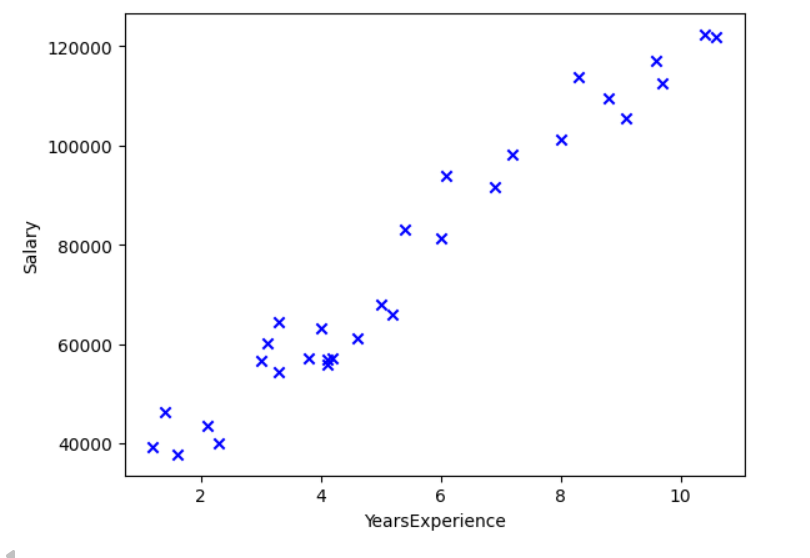
\includegraphics[scale=0.75]{img/201-1}

Ось простий приклад залежності між стажем роботи співробітників та їхньою заробітною платою. Чи можна передбачити другий параметр на основі значення першого?

Можна припустити, що залежність відповідає лінійній моделі.

$$y \approx \theta_1 \cdot x + \theta_2$$


Тут 
- $\theta_1$ це “нахил” лінії, та (slope)
- $\theta_2$ зсув. (intercept)

Чи можемо ми робити передбачення даних?

\begin{lstlisting}
import numpy as np

def build_line(plt, theta):
    xlim, ylim =(plt.gca().get_xlim(), plt.gca().get_ylim())
    plt.plot(xlim, [theta[0]*xlim[0]+theta[1], theta[0]*xlim[1]+theta[1]], 'C1')
    plt.xlim(xlim)
    plt.ylim(ylim)

plt = build_plot('../resources/Salary_dataset.csv', 'YearsExperience', 'Salary')
build_line(plt, np.array([9000, 25000]))
\end{lstlisting}


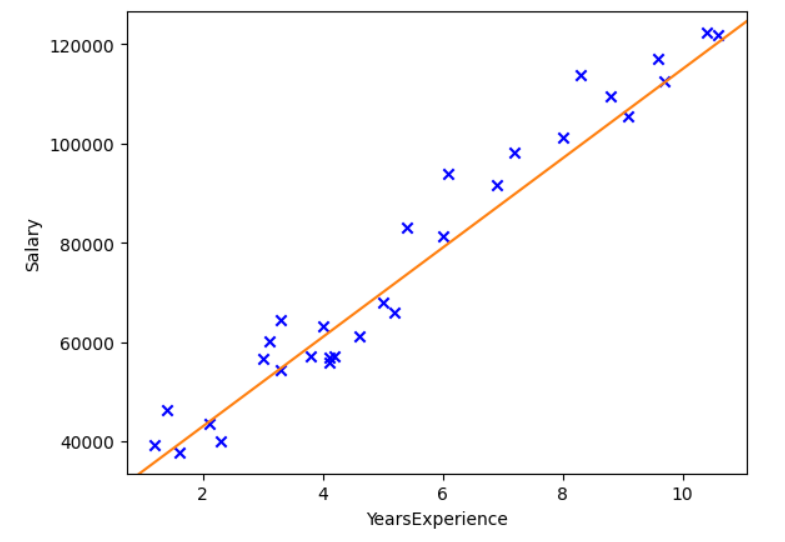
\includegraphics[scale=0.75]{img/201-2}

Ознака (feature) — це характеристика об'єкта, яка використовується моделлю для прийняття рішення. Цільова змінна (target) - це значення, яке модель повинна навчитися прогнозувати. У нашому прикладі, стаж працівника є ознакою (зазвичай у задачах машинного навчання їх значно більше, ніж одна), а заробітна плата - це цільова змінна.


\section{Градієнтний спуск.}

Припустимо, що прогнозована зарплата відповідає лінійній моделі. Як ми можемо знайти $\theta$? 

Є багато можливостей, але природною метою є мінімізація деякої різниці між цією лінією 
і спостережуваними даними, наприклад, квадратична втрата:

$$E(\theta) = \sum_{i}(\theta_{1}*x_{i} + \theta_{2} - y_{i} )^{2}$$

Тепер нам потрібно знайти параметри, які мінімізують значення функції $E(\theta)$.

$$minimize_{\theta}E(\theta)$$

Найкращий спосіб знайти значення функції $f(x)$, в якій її значення є мінімальним, — це знайти похідну. Ми починаємо з деякої точки і змінюємо вхідне значення в напрямку від'ємної похідної. У випадку багатозмінних функцій ми будемо використовувати часткові похідні.

Щоб знайти хороше значення $\theta$, ми можемо повторно робити кроки в напрямку 
негативних похідних для кожного значення. Ітерація:

$$ \theta_{1} := \theta_{1} - \alpha \frac{\delta}{\delta \theta_{1}} E(\theta_{1}, \theta_{2})$$

$$ \theta_{2} := \theta_{2} - \alpha \frac{\delta}{\delta \theta_{2}} E(\theta_{1}, \theta_{2})$$

де $\alpha$ — це невелике додатне число, яке називається розміром кроку.
Це алгоритм градієнтного спуску, основа сучасного машинного навчання.

Тут: 

$$\frac{\delta}{\delta \theta_{1}} E(\theta_{1}, \theta_{2}) = \sum_{i}2(\theta_{1}*x_{i} + \theta_{2} - y_{i} )*x_{i}$$

$$\frac{\delta}{\delta \theta_{2}} E(\theta_{1}, \theta_{2}) = \sum_{i}2(\theta_{1}*x_{i} + \theta_{2} - y_{i} )$$

Застосуємо градієнтний спуск (Gradient descent) до наших даних, спочатку нормалізувавши їх.

\begin{lstlisting}
def build_plot_normalized(file_path, x, y):
    data = pd.read_csv(file_path)
    x_nor = (data[x] - min(data[x])) / (max(data[x]) - min(data[x]))
    y_nor = (data[y] - min(data[y])) / (max(data[y]) - min(data[y]))
    plt.scatter(x_nor, y_nor, c='blue', marker='x')
    plt.xlabel(x)
    plt.ylabel(y)
    return plt

build_plot_normalized('../resources/Salary_dataset.csv', 'YearsExperience', 'Salary').show()
\end{lstlisting}


Візуалізуємо процес градієнтного спуску. Поки що, проведемо лише одну ітерацію.


\begin{lstlisting}
# Visualizing the gradient descent:

def get_data(file_path, x_name, y_name):
    data = pd.read_csv(file_path)
    return data[x_name], data[y_name]

def normalize_data(x):
    x_normalized = (x - min(x)) / (max(x) - min(x))
    return x_normalized

def gradient_descent(x, y, iters, alpha):
    theta = np.array([0., 0.])
    for t in range(iters):
        theta[0] -= alpha/len(x) * 2 * sum((theta[0] * x + theta[1] - y)*x)
        theta[1] -= alpha/len(x) * 2 * sum((theta[0] * x + theta[1] - y) )
    return theta 

def plot_fit(x, y, theta):
    plt.scatter(x, y, marker = 'x')
    xlim, ylim =(plt.gca().get_xlim(), plt.gca().get_ylim())
    plt.plot(xlim, [theta[0]*xlim[0]+theta[1], theta[0]*xlim[1]+theta[1]], 'C1')
    plt.xlim(xlim)
    plt.ylim(ylim) 

x, y = get_data('../resources/Salary_dataset.csv', 'YearsExperience', 'Salary')
x_normalized, y_normalized = normalize_data(x), normalize_data(y)

#first iteration
theta = gradient_descent(x_normalized, y_normalized, 0, 0.1)
plot_fit(x_normalized, y_normalized, theta)
\end{lstlisting}

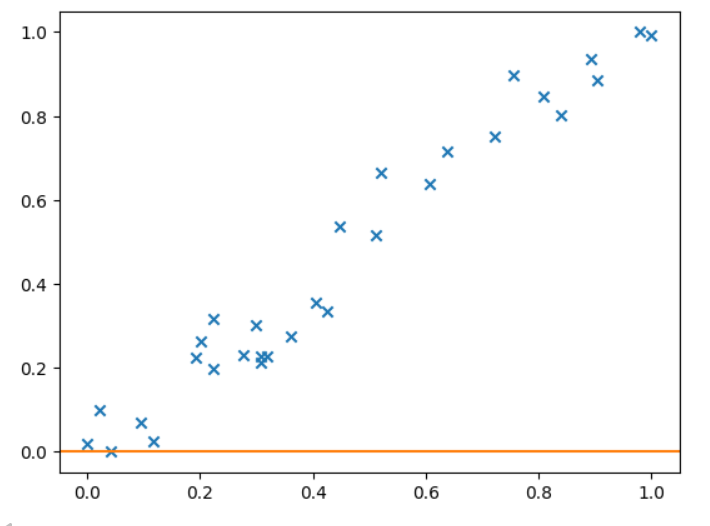
\includegraphics[scale=0.75]{img/201-3}

Як бачимо, на першій ітерації значення параметрів $\theta$ віддалені від бажаних. Проведемо іще декілька ітерацій.

\begin{lstlisting}
theta = gradient_descent(x_normalized, y_normalized, 2, 0.1) # change third parameter to see more iterations
plot_fit(x_normalized, y_normalized, theta)
\end{lstlisting}

Результат:

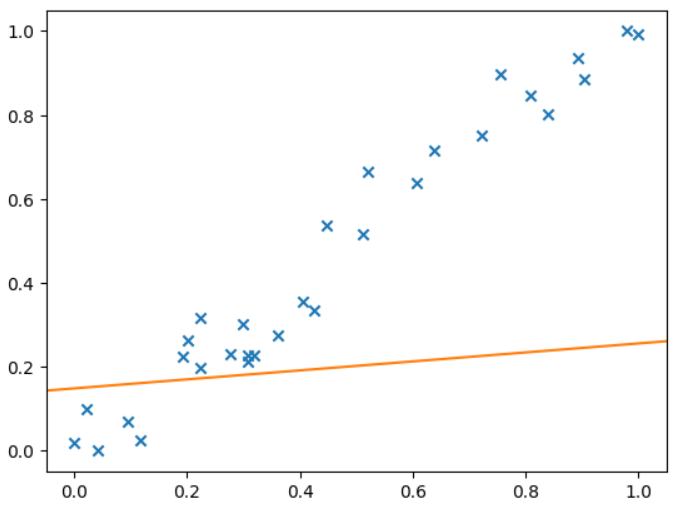
\includegraphics[scale=0.75]{img/201-4}


\begin{lstlisting}
theta = gradient_descent(x_normalized, y_normalized, 5, 0.1) # change third parameter to see more iterations
plot_fit(x_normalized, y_normalized, theta)
\end{lstlisting}

Результат:

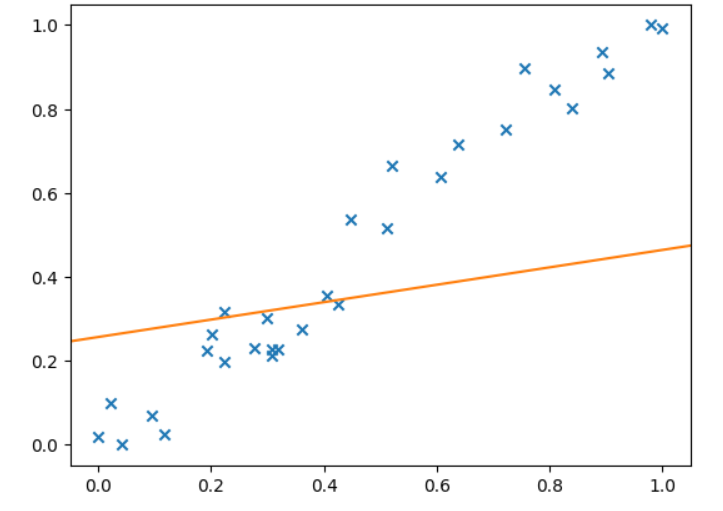
\includegraphics[scale=0.75]{img/201-5}


\begin{lstlisting}
theta = gradient_descent(x_normalized, y_normalized, 10, 0.1) # change third parameter to see more iterations
plot_fit(x_normalized, y_normalized, theta)
\end{lstlisting}

Результат:

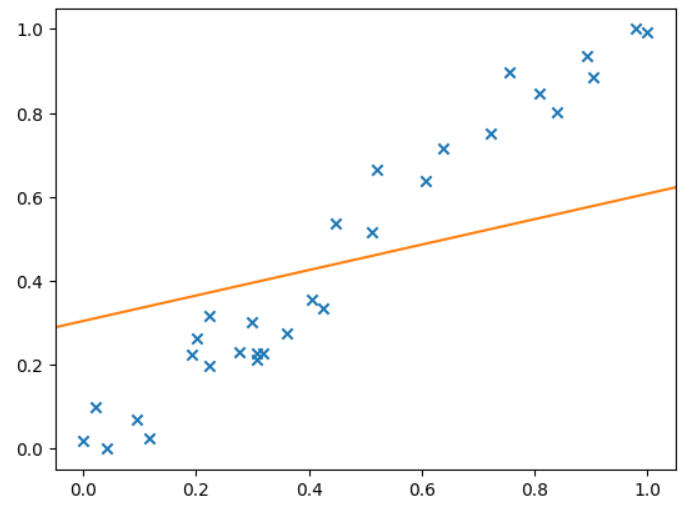
\includegraphics[scale=0.75]{img/201-6}


\begin{lstlisting}
theta = gradient_descent(x_normalized, y_normalized, 100, 0.1) # change third parameter to see more iterations
plot_fit(x_normalized, y_normalized, theta)
\end{lstlisting}

Результат:

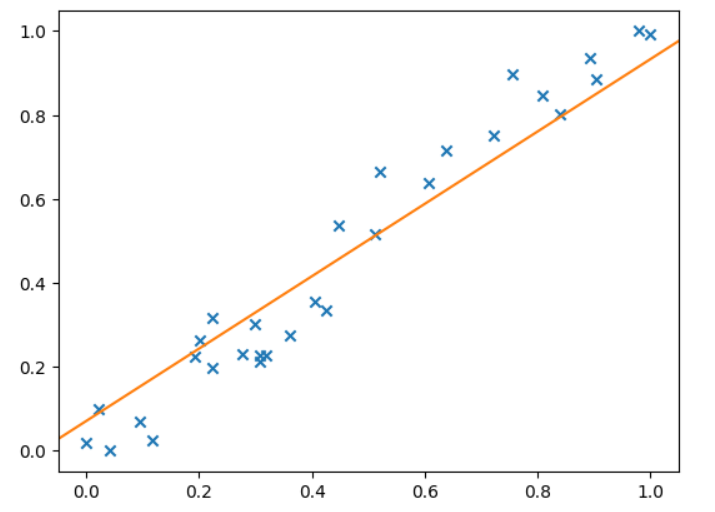
\includegraphics[scale=0.75]{img/201-7}

Після 100-ї ітерації ми наблизилися із нашою лінійною моделлю до реального розподілу. 

Ми також можемо візуалізувати процес зміни параметрів $\theta$:

\begin{lstlisting}
# Visualizing parameter updates

def gradient_descent_params(x, y, iters):
    thetas = []
    theta = np.array([0., 0.])
    alpha = 1.0
    for t in range(iters):
        thetas.append(theta.copy())
        theta[0] -= alpha/len(x) * 2 * sum((theta[0] * x + theta[1] - y)*x)
        theta[1] -= alpha/len(x) * 2 * sum((theta[0] * x + theta[1] - y) )
    return np.array(thetas)

def err(x, y, theta):
    return np.mean((np.outer(x, theta[:,0]) + theta[:,1] - y[:,None])**2,axis=0)

thetas = gradient_descent_params(x_normalized, y_normalized, 100)
plt.plot(thetas[:,0], thetas[:,1])
xlim, ylim =(np.array(plt.gca().get_xlim()), np.array(plt.gca().get_ylim()))
xlim += np.array([0,0.5])
ylim += np.array([-0.1, 0.1])

XX,YY = np.meshgrid(np.linspace(xlim[0],xlim[1],200), np.linspace(ylim[0], ylim[1],200))
ZZ = err(x_normalized.to_numpy(), y_normalized.to_numpy(), np.hstack([np.ravel(XX)[:,None], np.ravel(YY)[:,None]])).reshape(XX.shape)
#V = np.logspace(np.log(np.min(ZZ)), np.log(np.max(ZZ)), 30)
V = np.linspace(np.sqrt(np.min(ZZ)), np.sqrt(np.max(ZZ)), 25)**2
plt.clf()
plt.contour(XX,YY,ZZ, V, colors=('C0',))
plt.plot(thetas[:,0], thetas[:,1], 'C1-x')
plt.xlabel("theta1")
plt.ylabel("theta2")
\end{lstlisting}

Результат:

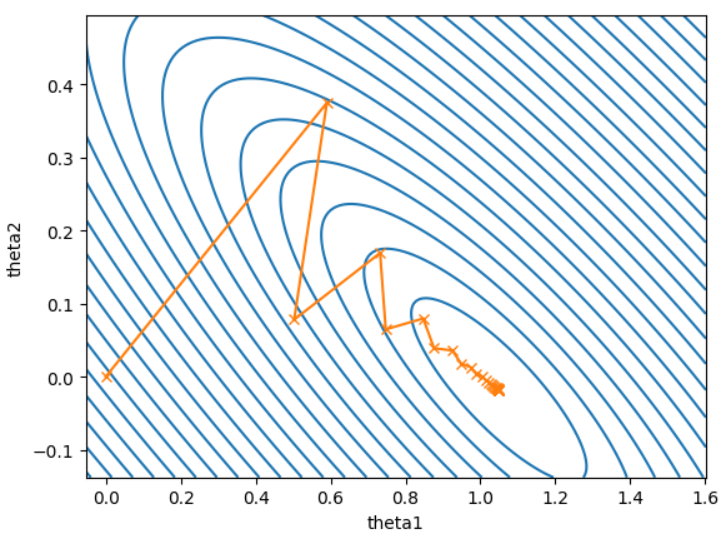
\includegraphics[scale=0.75]{img/201-8}

\subsection{Біблотека scikit-learn.}

Зробимо те саме лінійне прогнозування, використовуючи бібліотеку scikit-learn. Для того, щоб використати модель лінійної регресії, її спочатку потрібно імпортувати:

\begin{lstlisting}
from sklearn.linear_model import LinearRegression
\end{lstlisting}


Перетворимо наші дані в масиви numpy (саме з цими масивами і працює scikit-learn) та перетворимо вектор даних у матрицю за допомогою методу \verb|.reshape()|

\begin{lstlisting}
data = pd.read_csv('../resources/Salary_dataset.csv')
X = np.array(data['YearsExperience']).reshape(-1, 1)  
y = np.array(data['Salary'])  
\end{lstlisting}

\ding{43} Більшість алгоритмів бібліотеки scikit-learn очікують, що вхідні дані матимуть вигляд \verb|(кількість_об'єктів, кількість_ознак)|. Тобто, навіть якщо ознака лише одна, модель все одно хоче отримати матрицю, а не звичайний вектор. Саме тому і варто застосовувати метод \verb|.reshape()|.

Етап тренування моделі:

\begin{lstlisting}
model = LinearRegression()
model.fit(X, y)
\end{lstlisting}


Ми можемо отримати параметри theta:

\begin{lstlisting}
slope = model.coef_[0]       # theta_1
intercept = model.intercept_ # theta_2 
print("slope:", slope, "intercept:", intercept)
\end{lstlisting}

Та, зрештою, побудуємо лінію:

\begin{lstlisting}
X_line = np.linspace(X.min(), X.max(), 100).reshape(-1, 1)
y_line = model.predict(X_line)

plt.scatter(X, y, c='blue', marker='x')         
plt.plot(X_line, y_line)   # line
plt.xlabel("X")
plt.ylabel("y")
plt.title("Linear Regression Fit")
plt.show()
\end{lstlisting}


Весь код разом:

\begin{lstlisting}
import numpy as np
import matplotlib.pyplot as plt
from sklearn.linear_model import LinearRegression

data = pd.read_csv('../resources/Salary_dataset.csv')
X = np.array(data['YearsExperience']).reshape(-1, 1)  
y = np.array(data['Salary'])                

model = LinearRegression()
model.fit(X, y)

slope = model.coef_[0]       # theta_1
intercept = model.intercept_ # theta_2 
print("slope:", slope, "intercept:", intercept)

X_line = np.linspace(X.min(), X.max(), 100).reshape(-1, 1)
y_line = model.predict(X_line)

# plot 
plt.scatter(X, y, c='blue', marker='x')  
plt.plot(X_line, y_line)   # line
plt.xlabel("X")
plt.ylabel("y")
plt.title("Linear Regression Fit")
plt.show()
\end{lstlisting}

Результат:

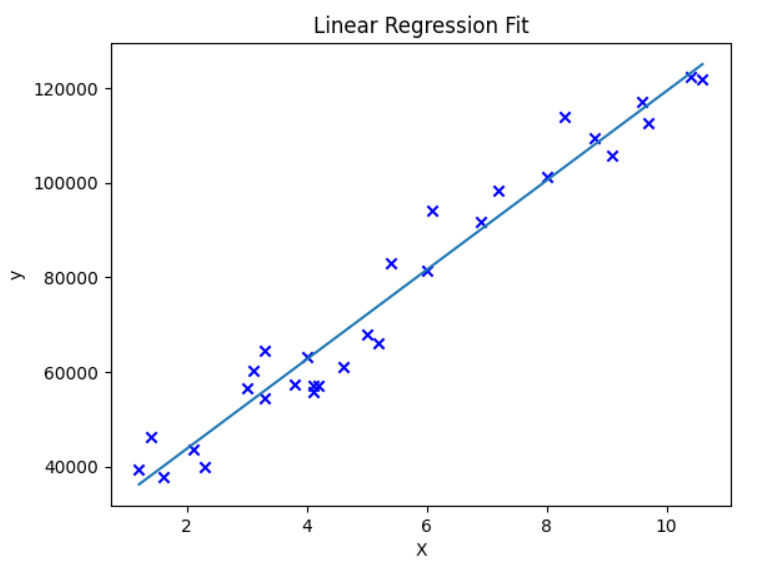
\includegraphics[scale=0.75]{img/201-9}

\section{Трохи більше про машинне навчання.}

Машинне навчання надає можливість автоматично встановлювати прогнозну модель на основі даних.

\textit{Термінологія}. Функція втрат: $l: y \times y \rightarrow \mathrm{R}$, вимірює різницю між прогнозом і 
фактичним результатом $$l(y',y)=(y'-y)^{2}$$

Канонічна задача оптимізації машинного навчання:

$$minimize_{\theta}\sum_{i}l(h_{\theta}(x^{i}), y^{i})$$

Практично кожен алгоритм машинного навчання має таку форму, просто вкажіть

\begin{itemize}
\item Що таке функція гіпотези?
\item Що таке функція втрат?
\item Як вирішити задачу оптимізації?
\end{itemize}

При застосування алгоритмів машинного навчання дані слід розбити на навчальні та тестову. Навчальна вибірка (Training Set) - це набір даних, який використовується для навчання моделі. Тестова вибірка (Test Set) використовується для перевірки якості вже навченої моделі. Під час тестування модель отримує дані, яких вона раніше не бачила. Це дозволяє оцінити, наскільки добре вона здатна узагальнювати знання та працювати з новими прикладами.

Можна виділити наступні основні етапи виконання алгоритму машинного навчання:

\begin{enumerate}
\item Збір даних. Отримання інформації з баз даних, файлів, вебресурсів, датчиків або інших джерел.
\item Попередня обробка даних. Очищення даних від помилок, пропущених значень, дублікатів та аномалій.
\item Виділення ознак. Вибір або створення характеристик, які використовуватимуться моделлю для навчання.
\item Поділ даних. Розбиття даних на навчальну та тестову вибірки.
\item Навчання моделі. Побудова математичної моделі на навчальних даних.
\item Оцінювання якості. Перевірка точності моделі на тестовій вибірці за допомогою відповідних метрик.
\item Використання моделі. Застосування навченої моделі для прогнозування нових даних.
\end{enumerate}


\subsection{Приклади алгоритмів машинного навчання.}

\begin{itemize}
\item Найменші квадрати: лінійна гіпотеза, квадратична втрата, (зазвичай) аналітичне 
рішення.
\item Лінійна регресія: лінійна гіпотеза.
\item Машина опорних векторів (support vector machine): лінійна або ядрова гіпотеза, втрата шарніра, etc.
\item Нейронна мережа: складена нелінійна функція, etc., (зазвичай) градієнтний 
спуск)
\item Дерево рішень (decision trees): ієрархічні півплощини, вирівняні по осі, жадібна оптимізація
\item Наївний Байєс: лінійна гіпотеза, спільна ймовірність за певних 
припущень незалежності, аналітичне рішення.
\end{itemize}



\ding{46} \textbf{Питання для самоконтролю.}

\begin{enumerate}
\item Що таке машинне навчання?
\item Чим машинне навчання відрізняється від традиційного програмування?
\item Які основні етапи побудови моделі машинного навчання?
\item Що таке навчальна вибірка?
\item Для чого використовується тестова вибірка?
\item Що таке ознака (feature)?
\item Що таке цільова змінна (target)?
\item Які основні типи задач машинного навчання існують?
\item Що таке навчання з учителем (Supervised Learning)?
\item Що таке навчання без учителя (Unsupervised Learning)?
\item Що таке навчання з підкріпленням (Reinforcement Learning)?
\item Чим задача класифікації відрізняється від задачі регресії?
\item Наведіть приклади задач класифікації.
\item Наведіть приклади задач регресії.
\item Що таке кластеризація?
\item Які практичні задачі можна розв'язувати за допомогою машинного навчання?
\item Що таке модель машинного навчання?
\item Що означає навчити модель?
\item Що таке прогнозування (prediction)?
\item Що таке лінійна регресія?
\item Для яких задач використовується лінійна регресія?
\item Який вигляд має рівняння простої лінійної регресії?
\item Що означає коефіцієнт нахилу (slope) у рівнянні лінійної регресії?
\item Що означає вільний член (intercept)?
\item Як інтерпретувати коефіцієнти лінійної регресії?
\item Що таке прогнозоване значення моделі?
\item Що таке похибка прогнозування?
\item Чому модель не завжди проходить через усі точки навчальної вибірки?
\item Що таке функція втрат (Loss Function)?
\item Для чого використовується середньоквадратична помилка (MSE)?
\item Як обчислюється середньоквадратична помилка?
\item Чому необхідно мінімізувати функцію втрат?
\item Що таке оптимізація моделі?
\item Що таке градієнтний спуск?
\item Яка основна ідея алгоритму градієнтного спуску?
\item Що таке градієнт функції?
\item Чому під час оптимізації рухаються у напрямку, протилежному градієнту?
\item Що таке швидкість навчання (learning rate)?
\item Як вибір швидкості навчання впливає на процес навчання моделі?
\item Які проблеми можуть виникнути при надто великому значенні learning rate?
\item Які проблеми можуть виникнути при надто малому значенні learning rate?
\item Що таке ітерація градієнтного спуску?
\item Коли алгоритм градієнтного спуску завершує свою роботу?
\item Чим Batch Gradient Descent відрізняється від Stochastic Gradient Descent?
\item Що таке Mini-Batch Gradient Descent?
\item Які переваги використання бібліотеки Scikit-learn для побудови моделей машинного навчання?
\item Яку роль відіграє бібліотека NumPy у задачах машинного навчання?
\item Як оцінити якість побудованої моделі лінійної регресії?
\item Чому важливо розділяти дані на навчальну та тестову вибірки?
\item Які обмеження має лінійна регресія та в яких випадках доцільно використовувати складніші моделі машинного навчання?
\end{enumerate}